\title{Um pouco de R na \textit{Newsletter}}
\subtitle{Nuvem de palavras}
\author{por Alessandro Samuel-Rosa}
\maketitle
\begin{wrapfigure}{l}{0.15\textwidth}
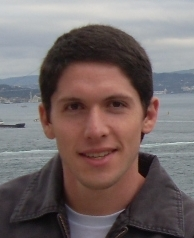
\includegraphics[width=0.15\textwidth]{figuras/foto-alessandro}
\end{wrapfigure}
O ambiente de análise de dados \R{} possui uma imensidade de funcionalidades que vão desde simples operações algébricas até a modelagem de complexas relações entre o solo e os fatores de formação do solo. Um bom exemplo do último caso é mostrado acima no artigo do Waldir, do Cesar e da Michele sobre a disciplina de mapeamento digital de solos ministrada na Universidade Federal Rural do Rio de Janeiro. Mas o que poucos sabem é que, sendo um ambiente de análise de dados, e não um simples software estatístico, quaisquer tipos de dados podem ser analisados no \R{}. Isso inclui dados contínuos, categóricos, imagens, vetores, volumes, 1D, 2D, 3D, 4D, áudio, vídeo, texto, e mais uma infinidade de possibilidades. Mas hoje vou me deter à apenas um destes tipos de dados, os dados textuais.
\subsection{Nuvem de palavras}
No presente número da \textit{Newsletter} da Comissão de Pedometria, uma novidade foi apresentada na página de abertura: um logo formado por uma nuvem de palavras.\\
\\
\emph{Uma nuvem de palavras, ou nuvem de tags, é uma representação visual de dados textuais onde a importância de cada palavra no texto é mostrada com o tamanho da fonte ou cor} \citep{wiki:2013}.\\
\\
Os dados textuais utilizados aqui são representados pelo conteúdo do seguinte vetor:
\begin{smallverbatim}
 > words <- c("pedometria pedometria pedometria
 pedometria solo estatística matemática sensores
 pedologia mapeamento gênese espaço variabilidade
 amostra dados métodos variação informática
 tecnologia programação script amostragem GPS
 satélite MDE pedólogo regressão geoestatística
 pedotransferência modelos resíduo incerteza
 computador mapas covariáveis tempo 3D função
 validação calibração SIG sistema predição
 interpolação ajuste curva rede neural árvore
 decisão classificação especialista erro
 correlação seleção automático paisagem logística
 simulação terreno atributo geologia clima imagem
 pixel escala resolução ensino pesquisa extensão
 agricultura ambiente precisão acurácia")
\end{smallverbatim}
A composição do vetor de dados textuais foi definida a partir da minha memória dos termos mais relacionados à pedometria. Como minha memória é falha e enviesada pelas minhas experiências pessoais, é provável que muitos outros termos poderiam ter sido incluídos. Sugestões são bem vindas para preparar o logo dos próximos números da \textit{Newsletter}. Além disso, outros dados textuais também podem ser analisados, como por exemplo o conteúdo textual de um artigo, livro ou até mesmo da \textit{Newsletter}. Como fazer isto é o que eu mostro abaixo.
\subsection{Instalando os pacotes necessários}
\label{subsec:pacotes}
Os pacotes necessários para a elaboração de uma nuvem de palavras, como aquela usada como logo da \textit{Newsletter}, são quatro: \texttt{wordcloud} \citep{Fellows:2013}, \texttt{tm} \citep{FeinererEtAl:2013}, \texttt{slam} \citep{HornikEtAl:2013}, e \texttt{RColorBrewer} \citep{Neuwirth:2011}. O pacote \texttt{wordcloud} é aquele que gera a nuvem de palavras usado como logo da \textit{Newsletter}. Já os pacotes \texttt{tm} e \texttt{slam} são dependências do pacote \texttt{wordcloud} usados na análise dos dados para a geração da nuvem de palavras. Para instalar e carregar estes pacotes basta usar os comandos:
\begin{smallverbatim}
> install.packages(c("wordcloud","tm", "slam",
"RColorBrewer"),
> repos = "http://cran.r-project.org")
> require(wordcloud)
> require(RColorBrewer)
\end{smallverbatim}
\subsection{Definindo a paleta de cores}
Depois de instalados e carregados os pacotes, define-se a paleta de cores usando o pacote \texttt{RColorBrewer}. São diversas as opções de paletas de cores do pacote \texttt{RColorBrewer}, cuja demonstração está além do objetivo deste artigo. Maiores informações podem ser encontradas acessando o endereço \url{http://colorbrewer2.org/}. No caso da nuvem de palavras usada como logo da \textit{Newsletter}, a paleta usada foi aquela identificada como \texttt{YlOrBr}, que varia entre as cores amarelo (\emph{yellow}), laranja (\emph{orange}) e marrom (\emph{brown}). O comando usado é o seguinte:
\begin{smallverbatim}
> pal <- brewer.pal(n = 9, name = "YlOrBr")
\end{smallverbatim}
\subsection{Gerando a nuvem de palavras}
Carregados os pacotes necessários, definidos os dados textuais e a paleta de cores, agora é possível invocar a função \texttt{wordcloud} para gerar a nuvem de palavras:
\begin{smallverbatim}
> wordcloud(words = words, min.freq = Inf,
random.order = FALSE, random.color = TRUE,
colors = pal, rot.per = 0.2, fixed.asp = TRUE)
\end{smallverbatim}
Os parâmetros fornecidos ao comando \texttt{wordcloud} definem o objeto do \R{} contendo os dados textuais (\texttt{words = words}), não havendo limite de frequência mínima para que um termo que aparece nos dados textuais seja apresentado graficamente (\texttt{min.freq = Inf}). Os termos são apresentados no gráfico em ordem decrescente de frequência (\texttt{random.order = FALSE}) e as cores da paleta (colors = pal) são atribuídas aleatoriamente (\texttt{random.color = TRUE}). Apenas 20\% dos termos podem ser apresentados graficamente na vertical (\texttt{rot.per = 0.2}), dando-se preferência pela apresentação gráfica com a relação de aspecto dos eixos x e y fixa (\texttt{fixed.asp = TRUE}).
\subsection{Salvando a nuvem de palavras como figura}
Depois de gerada a nuvem de palavras, existem diversas maneiras de salvar uma figura para usar, por exemplo, no cabeçalho da \textit{Newsletter}. A primeira opção é salvar um arquivo no formato *.pdf usando o seguinte comando:
\begin{smallverbatim}
> pdf(file = "wordcloud.pdf")
> wordcloud(words = words, min.freq = Inf,
random.order = FALSE, random.color = TRUE,
colors = pal, rot.per = 0.2, fixed.asp = TRUE)
> dev.off()
\end{smallverbatim}
A segunda opção é salvar um arquivo no formato *.png usando o seguinte comando:
\begin{smallverbatim}
> x11(width = 17/2.5, height = 7.5/2.5,
bg = "black")
> wordcloud(words = words, min.freq = Inf,
random.order = FALSE, random.color = TRUE,
colors = pal, rot.per = 0, fixed.asp = FALSE)
> savePlot(filename = "wordcloud-black.png")
> dev.off()
\end{smallverbatim}
Note que o arquivo salvo no formato *.png possui algumas peculiaridades, como por exemplo o uso do comando \texttt{x11()} para definir uma região de apresentação gráfica com $17/2.5$ polegadas de largura e $7.5/2.5$ polegadas de altura, com plano de fundo preto (\texttt{bg = "black"}). Além disso, nenhum termo foi permitido aparecer na vertical e a relação de aspecto dos eixos x e y foi mantida livre (\texttt{rot.per = 0} e \texttt{fixed.asp = FALSE}). Os produtos gráficos são mostrados pelas figuras \ref{fig:wordcloud} e \ref{fig:wordcloud-black}.\\
\\
\begin{figure}[htbp]
   \centering
   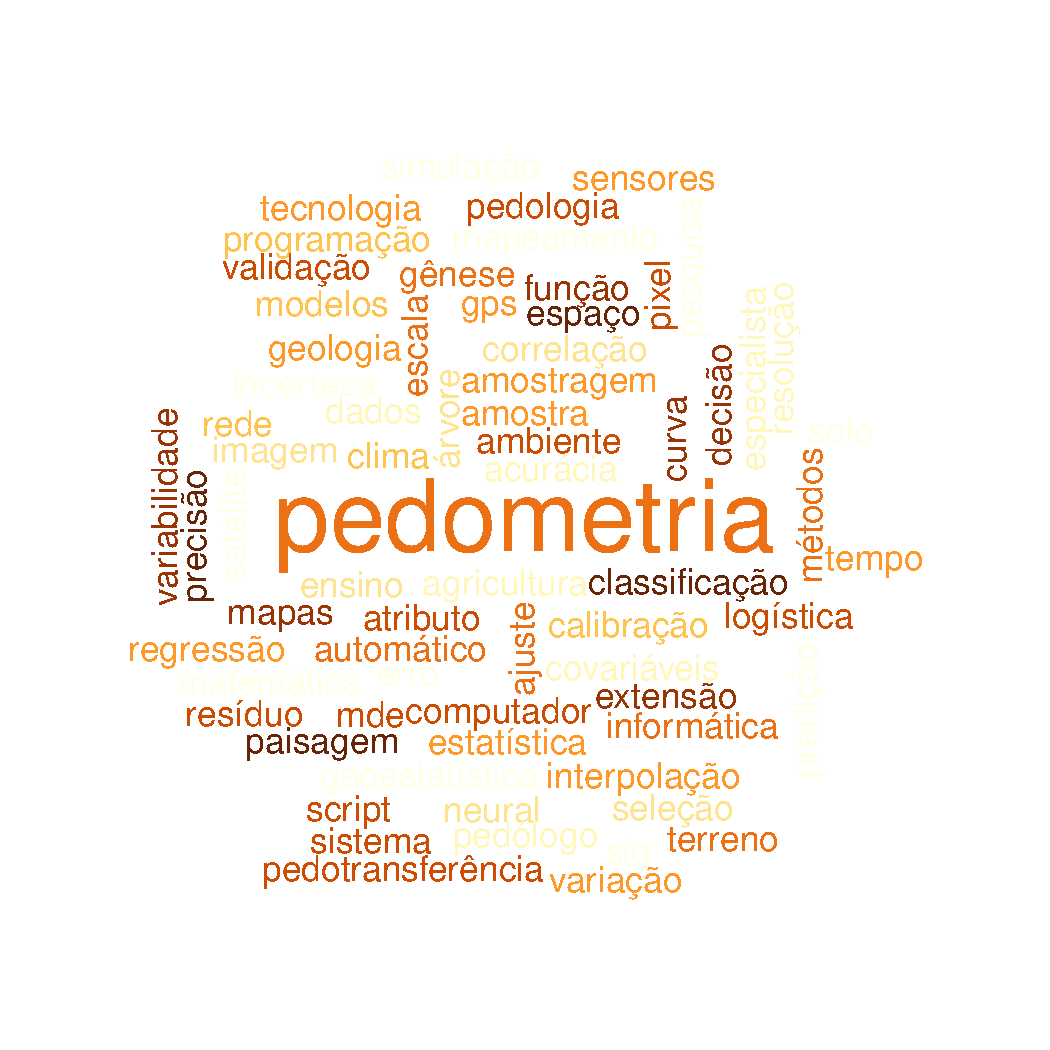
\includegraphics[scale=0.8]{figuras/wordcloud}
   \caption{Nuvem de palavras ligadas à pedometria com fundo branco e relação de aspecto fixa.}
   \label{fig:wordcloud}
\end{figure}
\noindent Diversas alterações podem ser feitas no produto gráfico final simplesmente alterando o conteúdo do vetor de dados textuais. Para aumentar ainda mais o tamanho do termo ``pedometria'' em relação aos demais termos, basta repeti-lo mais algumas vezes. Da mesma forma, se quisermos dar ênfase a outros termos, como por exemplo ``matemática'' e ``estatística'', basta repeti-los mais algumas vezes.\\
\\
\begin{figure}[htbp]
   \centering
   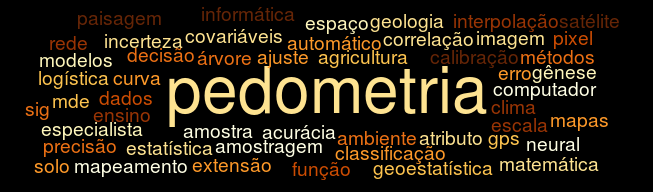
\includegraphics[scale=0.8]{figuras/wordcloud-black}
   \caption{Nuvem de palavras ligadas à pedometria com fundo preto e relação de aspecto livre.}
   \label{fig:wordcloud-black}
\end{figure}
\subsection{Um pouco de \R{} na \textit{Newsletter}}
Como eu disse no início deste artigo, existem diversos termos que poderiam ter sido acrescentados ao meu objeto contendo os dados textuais. Tais termos não foram incluídos simplesmente porque eu não lembrei deles ou porque não fazem parte do conjunto de termos que costumo relacionar à pedometria. É por este motivo que aqueles que gostarem de ver outros termos na nuvem de palavras que compõe o logo da \textit{Newsletter}, por favor, não exitem em entrar em contato pelo endereço de e-mail \email{alessandrosamuel@yahoo.com.br}. Ao mais aventureiros, o script usado no \R{} para produzir a nuvem de palavras pode ser baixado \href{http://goo.gl/tqGmI1}{clicando aqui} e usado para gerar novas e diferentes nuvens de palavras.
\begin{footnotesize}
\begin{thebibliography}{99}
\bibitem[Wikipedia (2013) Wikipedia]{wiki:2013}
Wikipedia (2013)
\newblock Tag cloud --- Wikipedia, The Free Encyclopedia.
\newblock \url{http://en.wikipedia.org/w/index.php?title=Tag_cloud&oldid=571203887} [Online; accessed 8-October-2013].
\bibitem[Fellows (2013) Fellows]{Fellows:2013}
I. Fellows (2013)
\newblock wordcloud: Word Clouds.
\newblock \url{http://CRAN.R-project.org/package=wordcloud} [R package version 2.4]
\bibitem[Feinerer \& Hornik (2013) Feinerer \& Hornik]{FeinererEtAl:2013}
I. Feinerer \& K. Hornik (2013)
\newblock tm: Text Mining Package.
\newblock \url{http://CRAN.R-project.org/package=tm} [R package version 0.5-9.1]
\bibitem[Hornik et~al. (2013) Hornik, Meyer \& Buchta]{HornikEtAl:2013}
K. Hornik, D. Meyer \& C. Buchta (2013)
\newblock slam: Sparse Lightweight Arrays and Matrices.
\newblock \url{http://CRAN.R-project.org/package=slam} [R package version 0.1-30]
\bibitem[Neuwirth (2011) Neuwirth]{Neuwirth:2011}
E. Neuwirth (2011)
\newblock RColorBrewer: ColorBrewer palettes.
\newblock \url{http://CRAN.R-project.org/package=RColorBrewer} [R package version 1.0-5]
\end{thebibliography}
\end{footnotesize}
\address{Alessandro Samuel-Rosa\\
  Universidade Federal Rural do Rio de Janeiro\\
  \url{soil-scientist.net}\\
  \email{alessandrosamuel@yahoo.com.br}}
%%% Local Variables: 
%%% mode: latex
%%% TeX-master: documento-principal.tex
%%% End: 